\newpage
\subsection{Arbeitspakete von Raphael Gregarek}
Im folgenden Abschnitt wird behandelt, wie Herr Gregarek den Marketing Mix, den Warenkorb, sowie den Bestellvorgangsprozess gelöst hat.

\subsubsection{Arbeitspaket 8: Warenkorb}
Zu Beginn wurde sich über die Funktionen und das Design des Warenkorbs Gedanken gemacht. Ziel war es, das die nötigen Funktionen verfügbar sind, zum Beispiel das Anzeigen von Artikeln mit diversen Eigenschaften sowie die Möglichkeit die Menge zu ändern als auch den Artikel vollständig aus dem Warenkorb zu entfernen. Dies wurde auch mit den anderen Gruppenmitgliedern kommuniziert, sodass mit der Programmierung des Warenkorbs fortgefahren werden konnte. Die \textit{Abbildung 37} zeigt das fertige Design des Warenkorbs. Es befinden sich noch 2 Buttons am unteren Ende die ermöglichen Artikel zu löschen oder den Bestellvorgang zu starten.\\

\textbf{Flyout Warenkorb}\\
\begin{figure}[H]
	\begin{center}
			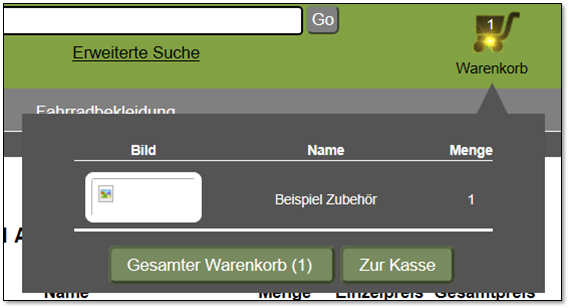
\includegraphics[width=95mm]{Bilder/warenkorb_flyout.png}
	\end{center}
	\caption{Flyout Warenkorb}
\end{figure}

Ähnlich wie die Profilverwaltung sollte auch der Warenkorb als Flyout aufrufbar sein um eine schnelle Ansicht der sich darin zu befindenden Artikel zu zeigen (siehe \textit{Abbildung 42}). Auch hier befinden sich wieder 2 Buttons. Der erste Button ermöglicht es den gesamten Warenkorb anzuzeigen. Dies ist aus dem Grund interessant, weil das Flyout unter Umständen nicht alle Artikel anzeigt. Das liegt daran, da das Flyout nur zur Übersicht sollte es klein sein und bei einer längeren Bestellung müsste man unter Umständen runterscrollen um den gesamten Warenkorb anzuzeigen. Dies wäre unübersichtlich und wenig hilfreich. Der zweite Button führt weiter zur Kasse, wo die Bestellung abgeschlossen wird. Das Warenkorbsymbol  (siehe \textit{Abbildung 43}) am oberen Teil des Webshops zeigt an, wie viele Artikel sich schon im Warenkorb befinden. Der restliche Teil des Warenkorbs wurde vom Gruppenmitglied Benedikt Brüntrup übernommen.

\begin{figure}[H]
	\begin{center}
			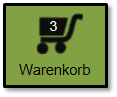
\includegraphics[width=25mm]{Bilder/Warenkorb_symbol.png}
	\end{center}
	\caption{Flyout Warenkorb}
\end{figure}

\subsubsection{Arbeitspaket 9: Bestellvorgang}
Große Teile wurden auch hier von Benedikt übernommen, sodass letztlich noch die Auflistung der bisherigen Bestellungen und die Möglichkeit der Stornierung implementiert wurden. Dazu wurden in der Klasse Bestellungen Methoden mit Datenbankanfragen erstellt. Da das Design im gesamten Webshop gleich ist, konnten die Style Anweisungen zum Teil vom Warenkorb übernommen werden.

\subsubsection{Arbeitspaket 10: Erstellung eines Marketing Mix}
Dieser Teil beschreibt wie der Marketing Mix erstellt wurde, beziehungsweise welche Teilschritte nötig waren um den Marketing Mix umzusetzen.\\
Zu Beginn wurde die Zielgruppe definiert sowie eine Marktanalyse angefertigt. Diese kann als Grundlage für den Marketing Mix angesehen werden und nur so ist es möglich die richtige Strategie für das eigene Unternehmen zu finden. Denn wenn man nicht weiß an wen das Produkt gerichtet ist und vor allem wie die Marktsituation auch in Hinblick auf die Zukunft ist, ist ein Marketing Mix ohne dieses Wissen wahrscheinlich hinfällig beziehungsweise weniger hilfreich. Nur mit einer Vorarbeit lässt sich eine feste Strategie planen, die auch zielführend ist.\\
Danach wurde der Marketing Mix erstellt. Wie für ihn üblich wurden die 4Ps (Produktpolitik, Preispolitik, Distributionspolitik und Kommunikationspolitik) der Reihe nach abgearbeitet. Dabei wurde in der Kommunikationspolitik nur auf die Online Vermarktung eingegangen, da dies auch in der Aufgabenstellung gefordert war. Einzig die Aufgabe nur den Großraum OWL anzusprechen wurde in den Hintergrund gerückt, da es online schwer ist klare Grenzen zu ziehen. Dies wurde auch im Marketing Mix berücksichtigt. \\

\textbf{Marktanalyse – Grundlage des Marketing Mix}\\

\small{\textbf{Die Zielgruppe festlegen}}\\
Als Zielgruppe selber wird jeder Mitbürger definiert, der in der Lage ist ein Fahrrad zu fahren oder eben jenes zu erwerben. Als Gruppe könnte auch nur der Großraum OWL wie in der Aufgabenstellung gefordert wird, als Zielgruppe definiert werden, jedoch ist es aufgrund eines Onlinemarketings und der Betreibung eines Webshops unmöglich nur den Großraum OWL als Zielgruppe zu nennen. Diese beiden Faktoren stehen gerade für die Globalisierung und vergrößern so die Zielgruppe ungemein. Die Grenzen des Webshops sind seine Lieferbedingungen, also die Lieferung der Artikel in bestimmte Länder. Und die GBI beschränkt sich hierbei auf Deutschland. Als weiteren Faktor ist auch die Sprache zu nennen. Denn durch die Wahl der Sprache im Webshop werden schon Menschen ohne deutsche Sprachkenntnisse ausgeschlossen, sodass diese auch nicht die Zielgruppe sein können.
Zu beachten ist auch die Produktplatte, die die GBI zu bieten hat. Sie hat vor allem Sportfahrräder und Mountain Bikes im Angebot. Die Zielgruppe auch wenn dies etwas stereotypisch ist, sind somit jüngere Männer. Natürlich verkauft die GBI die Fahrräder auch an andere Gruppen, jedoch wird der Großteil eben an die eben genannte Gruppe gehen, wobei der Begriff jung sehr weit gefasst werden kann. Gerade im Hinblick auf die E-Bikes kann sich die Käufergruppe sehr schnell ändern.\\

\small{\textbf{Marktgröße}}\\
Hier sind verschiedene Aspekte zu beachten:
\begin{enumerate}

	\item \textbf{Die Marktgröße – wie groß ist der Markt in der Gegenwart}
	\begin{figure}[H]
		\begin{center}
			\fbox{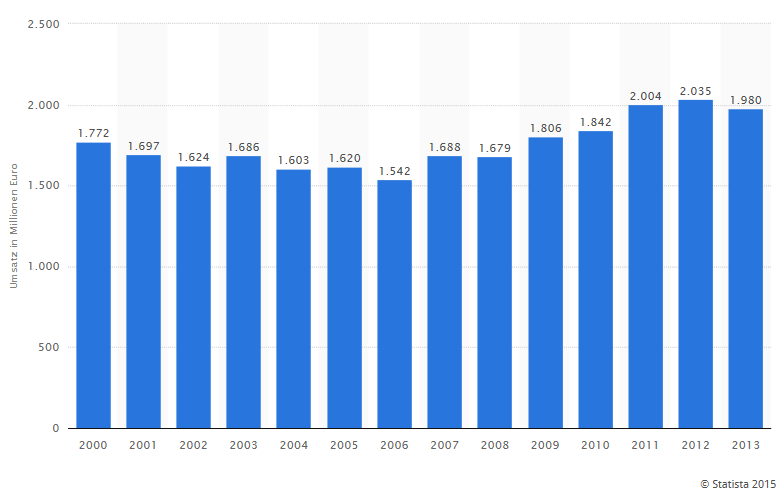
\includegraphics[width=125mm]{Bilder/umsatz_fahrrad_verkaeufe_de.png}}
		\end{center}
		\caption{Umsatz von Fahrradverkäufen in Deutschland}
	\end{figure}
	%Bildquelle: http://de.statista.com/statistik/daten/studie/154152/umfrage/umsatz-durch-fahrradverkaeufe-in-deutschland-seit-2000/
	
Das vergangene Jahr war für den Fahrradmarkt in Deutschland ein sehr starkes und bestätigt den groben Trend im Diagramm. Während von 2000 bis 2006 ein negativer Trend zu beobachten war, ist aber 2007 ein durchweg positiver Weg zu beobachten. Lediglich 2013 war sehr Umsatzschwach. 2014 wurden etwa 4,1 Millionen Fahrräder verkauft (inklusive E-Bikes) was einem Umsatz von 2,16 Milliarden Euro entspricht. Wichtig für die GBI ist auch der E-Bike Markt. In Deutschland gibt es momentan etwa 2,1 Millionen E-Fahrräder.

	\item{\textbf{Marktwachstum und –Dynamik – der Trend des Marktes}}
	
Der Markt ist in einer Wachstumsphase und das besonders bei den E-Fahrrädern. Ein Umsatzplus 2014 im zweistelligen Bereich macht dies deutlich. Aber auch der der Markt für nicht elektrische Fahrräder erfährt ein konstantes Wachstum. Somit erlebt der gesamte Markt einen positiven Trend, der auch von dem oben gezeigten Diagramm bestätigt wird.
Einen gesonderten Blick auf den E-Bike Markt sollte auf jeden Fall geworfen werden. Hier ist ein großes Wachstum in den nächsten Jahren zu erwarten, wenn man die momentane Situation zu Grunde legt. Gegenüber dem Vorjahr ein Plus von 17 Prozent ist eine sehr beachtliche Steigerung. Der Anteil der E-Fahrräder am gesamten Markt beträgt mittlerweile 12 Prozent.

	\item{\textbf{Marktpotenzial – Chancen des Marktes}}
	
Der Fahrradmarkt in Deutschland hat gute Chancen weiter zu wachsen. Dies hat verschiedene Gründe, die in sehr unterschiedlichen Bereichen liegen. Zum einen ist die Natur zu nennen. Damit ist gemeint, dass viele Menschen ihre Lebensweise ändern um die Natur weniger zu belasten. Das fängt damit an den Weg zur Arbeit mit dem Rad zu fahren. Dies tun einige der Natur zur Liebe andere sparen sich somit das Benzin, das für das Auto nötig wäre oder das Ticket für die Bahn oder den Bus. Das Fahrrad wird auch gerne als Sportmittel genutzt oder einfach dafür sich in der Umwelt zu bewegen.
Chancen sind vor allem im E-Fahrrad Markt. Mittlerweile werden auch jüngere Menschen mit anderen Modellen wie E-Mountainbikes angesprochen, was großen Anklang findet.
Die Entwicklung von E-Bikes sollte auch kritisch betrachtet werden. Im Moment wächst der Markt stetig, da es ein relatives neues Produkt ist. Die Gefahr, dass es nur eine Blase ist, die in naher Zukunft platzt ist eine durchaus denkbare  Möglichkeit. Jedoch sieht der momentane Blick in die Zukunft rosig aus, was das sehr starke Wachstum des E-Bike Marktes bestätigt. Dennoch muss immer im Blick sein, dass das Interesse nach E-Bikes sinken könnte.

\end{enumerate}
\textbf{Marketing Mix}\\

\small{\textbf{Aufgabenstellung}}\\
Dieser Abschnitt behandelt den Marketing Mix für den Großraum OWL. Bei dem Marketing Mix wurde besonders aufgrund des Webshops auf die Online-Vermarktung eingegangen.\\

\small{\textbf{Produktpolitik}}\\
Die GBI hat schon eine breite Palette an Fahrrädern und Zubehör zu bieten. Lediglich der Bereich der E-Bikes wird momentan erschlossen. Das Design sollte ähnlich den der bisherigen Modelle gewählt werden um auch bei den neuen Produkten einen Wiedererkennungswert zu generieren. Wenn möglich sollte das Fahrrad bzw. E-Bike das gleiche Aussehen haben und sich nur durch die notwendigen Eigenschaften unterscheiden, was ein E-Bike zu einem E-Bike macht.\\
Da der Webshop neu ist, könnte das Verpackungsdesign an das Unternehmen angepasst werden. Den Namen der Firma oder das Logo selber könnte an der Außenseite zu finden sein. So kann man sich von der Konkurrenz absetzen und schon beim bloßen Ansehen des Pakets wird das Unternehmen GBI sichtbar. Jedoch ist auch auf eine schlichte Verpackung zu achten, da die GBI Qualität vorlebt und dies muss nicht durch ein übertriebenes Verpackungsdesign zu Nichte gemacht werden.\\

\small{\textbf{Preispolitik im Marketingmix}}\\
Für die Preispolitik muss die GBI einige Faktoren berücksichtigen bevor sie sich letztendlich festlegt. Die GBI ist im Fahrradbereich ein bekanntes Unternehmen und in Teilbereichen sogar weltweiter Marktführer. Die Bereiche sind Sporträder und Mountain Bikes im Privatkundenumfeld und im geschäftlich öffentlichen Umfeld, der Spitzensport. Damit ist die GBI nicht gezwungen eine aggressive Preisstrategie zu fahren um Bekanntheit zu erlangen. Dies ist auch ein enormer Vorteil der GBI. Sie kennen den Markt schon und wissen durch ihre Erfahrung welcher Preis der Kunde bereit ist für ihre Produkte zu zahlen.

Der Webshop ist allerdings ein neuer Teilbereich und so sollten wenigstens für einen bestimmten Zeitraum besondere Angebote für Fahrräder und Ersatzteile gemacht werden. Der Webshop besitzt auf der Startseite schon erste Angebote. Dies sollte auch auf bestimmte Zeit so fortgeführt werden. Der Slogan \glqq Fahrrad des Tages\grqq{} generiert eine besondere Stellung des Fahrrads im Webshop und lenkt die Aufmerksamkeit auf dieses Produkt.

Der Verbraucher hat durch das Internet die Möglichkeit die Preise für jedes Produkt zu vergleichen und die GBI muss sich in diesem Bereich neu aufstellen, da Sie hier noch nicht mit einem eigenen Webshop vertreten war. Angebote helfen hierbei die Marke im Internet bekannter zu machen. Zu beachten ist jedoch auch die Philosophie für die, die GBI, steht. Der Fokus des Unternehmens ist auf Qualität, Stärke und Leistung festgelegt. Dies bedeutet auch, dass der Kunde von vornherein erwarten kann ein einwandfreies, qualitativ hochwertiges Produkt zu bekommen. Der Preis sollte sich also nicht im unteren Bereich des Marktes befinden. Dafür ist der Name zu bekannt, als das die GBI hier einen Preiskampf fahren muss. Der Webshop hat auch einen nicht unwichtigen Vorteil gegenüber z.B. Fahrradgeschäften. Der Verkaufsraum beziehungsweise auch der Verkäufer oder Ausstellungsstücke fallen im Internet weg. So spart man beachtliche Kosten die eine Drückung des Preises nach unten ermöglichen.

Die Kategorie E-Bikes ist ein neuer Bestandteil der Produktpalette und die GBI muss sich hier noch beweisen, dass sie auch in der Lage sind die gewohnten GBI Standards auf die neuen Produkte zu übertragen. Preislich sollte die GBI hier auch die direkten Konkurrenten im E-Bike Premiumsegment unterbieten um möglichst schnell einen Marktanteil zu generieren.

Die GBI sieht im Webshop zwei Liefermöglichkeiten. Zum einen der Standardversand. Die Kosten betragen üblicherweise 4€. Übersteigt der Wert der gekauften Waren eine bestimmten Wert, im Falle hier 25€, so fallen die Versandkosten weg. Die Idee beruht darauf, den Kunden nach Möglichkeit zu einem größeren Einkauf zu locken, um doch noch den festgelegten Wert zu überschreiten. Dies ist vor allem bei kleineren Produkten wie zum Beispiel bei Zubehör der Fall. Der kostenfreie Versand ist ein Anreiz mehr einzukaufen als man es eigentlich vorhatte. Die zweite Liefermöglichkeit ist für die GBI typisch. Es wird ein Expressversand für 13€ angeboten, der eine sehr schnelle Lieferung garantiert. Im Hinblick auf die Kernkompetenzen des Unternehmens, Qualität und Leistung,  ein guter Schritt, da diese beiden Kompetenzen weiter ausgebaut werden können. Bei den Zahlungsbedingungen geht die GBI kein Risiko ein und vertraut der Vorkasse und dem Bankeinzug. Der Bankeinzug ist vor allem im Deutschen Raum eine sehr beliebte Zahlungsart, weil hier der Kunde lediglich einmalig seine Bankdaten hinterlegen muss, auch wenn er mehrere Bestellungen tätigt und das Unternehmen selbst das Geld von dem Konto des Kunden abbucht.\\

\small{\textbf{Distributionspolitik}}\\
Bei der Distributionspolitik gibt es drei Wege das Angebot an der Kunden zu tragen. Die Möglichkeiten sind über Vermittler, Franchise oder als Direktvertrieb. Durch den neugeschaffenen Standort Höxter und den damit verbundenen Webshop fallen sowohl das Franchise als auch der Vermittler weg. Der Direktvertrieb bietet eine wahnsinnige Kundennähe und eine intensive Beratung. Vor allem bei Fahrrädern ist dies eine gute Idee, da diese sich teilweise sehr unterscheiden, und so kann der Kunde individuell beraten werden. Das fördert den Kundenkontakt und so auch auf Wünsche/Verbesserungen der Kunden eingegangen werden. Ein weiterer nicht unwichtiger Punkt, der für den direkten Vertriebsweg spricht, sind die Kosten. Sowohl Vermittler als auch Franchiseunternehmen möchten Geld verdienen und dadurch muss bei gleichbleibendem Gewinn der Verkaufspreis angehoben werden. Durch das Wegfallen dieser Kosten hat die GBI verschiedene Möglichkeiten das eingesparte Geld zu nutzen. Generell günstigere Preise oder gleichbleibende Preise bei einer höheren Gewinnspanne, vorausgesetzt die abgesetzte Menge bleibt gleich.

\begin{figure}[H]
	\begin{center}
			\fbox{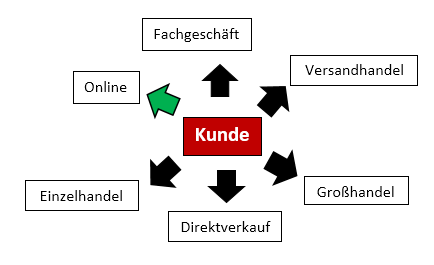
\includegraphics[width=90mm]{Bilder/vertriebskanaele.png}}
	\end{center}
	\caption{Die Vertriebskanäle im Überblick}
\end{figure}

Der nächste Schritt ist die Festlegung des Vertriebskanals der GBI. Hier sollte die Wahl auf dem Onlinehandel liegen. Der eigens angelegte Webshop eignet sich hervorragend um die Produkte der GBI anzubieten. Dafür wurde dieser schließlich angelegt. Die Angebote des Tages auf der Hauptseite sind eine gute Möglichkeit vor allem zur Eröffnung des Shops um möglichst viele Kunden auf die Webseite zu locken, damit der Bekanntheitsgrad steigt. Hier spielt auch der \glqq Click-Counter\grqq{} mir rein, der die Anzahl der Seitenaufrufe zeigt. Somit ist der Webshop möglicherweise bei Suchmaschinen schneller zu finden, da er schon viele Aufrufe generiert hat.

Die GBI muss jedoch auch bedenken, dass die Festlegung auf nur einen Vertriebsweg durchaus problematisch werden könnte. Sie ist durch den einen Vertriebsweg sehr abhängig von ihm. Daher sollte man nach Start des Shops die Verkaufszahlen beachten und den Markt weiter beobachten, ob es nicht sinnvoll wird, den einen oder anderen Vertriebskanal dem Unternehmen hinzuzufügen. Positiv bei der Wahl auf nur einen Kanal zu setzen ist die Tatsache, dass dies enorme Kosten spart. Denn bei den anderen Vertriebswegen gibt es immer mindestens eine handelnde Instanz, die Kosten verursacht, sei es nun das Fachgeschäft oder der Versandhandel.

\begin{figure}[H]
	\begin{center}
			\fbox{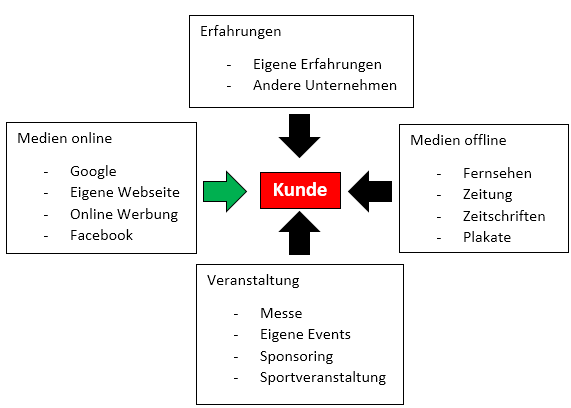
\includegraphics[width=90mm]{Bilder/Werbemoeglichkeiten.png}}
	\end{center}
	\caption{Werbemöglichkeiten im Überblick}
\end{figure}

\small{\textbf{Kommunikationspolitik}}\\
Die GBI wird von vornerein auf die Online Vermarktung setzen. Dies ist eine klare Ausrichtung. Dadurch wird die Kommunikationspolitik lediglich dieses Thema behandeln.

Die Marke GBI ist bekannt. Dies liegt daran, dass die Produkte der GBI in Spitzensport genutzt werden und dadurch die Öffentlichkeit aufmerksam wurde. Zudem sollten wieder die Kernkompetenzen genutzt werden. Qualität und Leistung. Dafür steht die GBI und das müssen auch potentielle Kunden wissen. Daraus resultiert auch die Vorgabe für die Werbung. Die Produkte sind qualitativ hochwertig und nicht minder sollte die Vermarktung sein. Das bedeutet zwar höhere Marketingkosten, jedoch ist das für das Image wichtig, da Kunden sowas miteinander assoziieren. Das Online Marketing kann auf verschiedene Weise genutzt werden. Durch die Festlegung der Zielgruppe im oberen Abschnitt, fällt die Vermarktung leichter. Denn nur wenn die GBI weiß, wer als Kunde geeignet ist, kann sie passgenau für ihre Produkte werben. Die GBI hat nun verschiedene Möglichkeiten ihre Produkte beziehungsweise den Webshop online zu vermarkten. Im Folgenden befindet sich eine grobe Übersicht:
\begin{enumerate}
	\item Marketing über E-Mail
	\item Marketing mithilfe von Suchmaschinen
	\item Schalten von Bannerwerbungen auf Webseiten
	\item Affiliate-Marketing
	\item Social Media Marketing
	\item Einbindung der Produkte in andere Webshops
	\item Der eigene Webshop beziehungsweise die eigene Webseite
\end{enumerate}

Für die GBI scheinen die Kategorien 1, 2, 3 und 5 am sinnvollsten zu sein. Dies ist der Tatsache geschuldet, dass zum einen nicht zwangsweise jede Kategorie beansprucht werden muss und zum anderen das die Kategorien 6 und 7 momentan noch unmöglich beziehungsweise nicht sehr sinnvoll erscheinen. Der Webshop befindet sich momentan im Aufbau und hat noch keine Bekanntheit. Von einer Webseite ist seitens der GBI keine Rede, weswegen diese Möglichkeiten erstmal wegfallen.

Die Marketing Methode über die E-Mail ist im Online Marketing eine lange bekannte und beliebte Variante. Man könnte denken, dass über soziale Netzwerke mehr Menschen erreicht werden aber letztlich ist es so, dass über 95\% der Internetnutzer ein E-Mail Konto besitzen und nur eine weitaus geringere Personenanzahl einen Social Media Account. Darüber hinaus nutzen Menschen nicht nur eine Social Media Seite beziehungsweise sind sie in manchen gar nicht aktiv. Ein E-Mail Konto ist unabhängig vom jeweiligen Anbieter.  Zudem sieht sich ein potentieller Kunde eher eine E-Mail an als einzelne Nachrichten auf einer Social Media Seite, wo förmlich eine Nachrichtenflut herrscht. Das wichtigste für die GBI ist einen Stamm an E-Mail Adressen aufzubauen. Wie dies für die GBI geschieht muss sie selber wissen. Über Offline Events können E-Mail Adressen gesammelt werden aber auch über die eigene Webpräsenz. Oder über die Social Media Seiten der Firma. Wichtig ist, dass vom potentiellen Kunden eine Einwilligung geholt wird. Rechtlich ist die GBI auf der sicheren Seite wenn sie nach dem Double Opt-In Verfahren arbeitet. Zusätzlich sollte noch das Impressum in der Mail vorhanden sein, sowie eine Möglichkeit sich wieder vom Newsletter abzumelden. Über die E-Mail Methode weiß die GBI, dass sie Kunden anspricht, die auch wirklich reges Interesse an dem Produkt zeigen, da sie sich für den Newsletter extra angemeldet haben.

Die zweite Möglichkeit ist die der Suchmaschinen. Bevor die GBI auf den ersten Seiten der Suchergebnisse erscheint wird dies etwas dauern. Beschleunigen lässt sich dies mit den AdWords von Google. Mit AdWords kann sich die GBI Stichwörter kaufen. Wenn nach diesem Stichwort nun gesucht wird taucht die GBI weiter oben in den Suchergebnissen auf. Je nach Stichwort kann dies aber ein teures Unterfangen sein. Zudem dauert es zu Start des Marketings mit AdWords einige Zeit bis die GBI vorne auftauchen wird. Eine andere Möglichkeit ist die der Search Engine Advertising (SEA). Hier bezahlt die GBI für eine Anzeige die neben den Suchergebnissen auftaucht. Gerade zu Beginn eine sinnvolle Alternative, da sich die Anzeige schon auf der ersten Suchergebnisseite befinden könnte. Letztlich sollte die GBI aus einer Mischung aus beidem abzielen. Jedoch kosten beide sehr viel Geld aber bieten ein enormes Potenzial.

Die nächste Art des Online Marketings ist die der Bannerwerbung. Grob unterschieden wird hier zwischen statischen, HTML-, Bild- und Text- sowie animierten Werbebannern. Es gibt sicherlich noch weitere Varianten, doch die eben genannten sind die Bekanntesten. Die Werbung wird auf beliebigen Webseiten geschaltet. Für die GBI bieten sich natürlich Fahrradseiten an, auch die im Bereich des Spitzensports. Im Sinne der Region OWL sollte auch auf regionalen Webseiten mit Bannern geworben werden. Je nachdem wie oft der Banner erscheint oder auf ihn geklickt wird, erhöhen sich die Kosten. Für die Webseiten der Region OWL sollte die GBI aber definitiv über die Bannerwerbung nachdenken.

Für das Social Media Marketing ist generell ein eigener Auftritt beziehungsweise eine eigene Seite sinnvoll. Die großen beiden Vertreter in der Branche sind Facebook und Twitter. Unabhängig auf welcher Seite sich die GBI nun präsentieren wird muss sie aktiv ihre Seite betreiben. Die eigene Seite ist weniger attraktiv, wenn sie nicht regelmäßig aktualisiert wird oder nur selten genutzt wird. So verlieren Kunden schnell das Interesse und werden den Auftritt nicht länger verfolgen. Besonders in Fahrradforen und Foren im Bereich OWL sollte die GBI auch aktiv werden. Dabei sollte sie nicht nur aktiv Werbung für ihre Produkte machen sondern auch potentiellen Kunden helfen. Das richtige Produkt empfehlen, aufzeigen was das Produkt besser macht aber auch ehrlich sein. So bekommt die GBI auch Feedback und kann dieses nutzen um sich selber ständig zu verbessern. Das Internet ist transparent und Fehltritte können fatale Folgen haben. So ist das Social Media Marketing nicht nur als Verkaufs- und Werbemöglichkeit zu sehen, sondern auch als Feedback- und Entwicklungsplattform. Um sehr schnell eine große Gemeinschaft aufzubauen wird der GBI empfohlen auf den Social Media Seiten fachbezogene Beiträge, Gewinnspiele und Rabattangebote anzubieten. Dies fördert das Wachstum der Gemeinschaft und verschafft in kürzester Zeit eine größere Beliebtheit. Gerade als weltweit agierendes Unternehmen, wie die GBI eines ist, wird sie schnell Zuspruch finden. Doch auch Vorsicht ist geboten. Qualität steht immer vor Quantität und das gerade bei der GBI. Lieber sollte sie in regelmäßigen Abständen die Seite aktualisieren als jede Stunden etwas zu verfassen.\\

\small{\textbf{Fazit des Marketing Mix}}\\
Mit diesem Marketing Mix hat die GBI eine Möglichkeit ihre Bekanntheit im deutschen Raum, insbesondere den Großraum OWL zu erweitern. Es wurden sowohl Chancen als auch Risiken gegenübergestellt und konkrete Punkte angesprochen wie die GBI den Webshop einbinden kann. Die 4Ps wurden nacheinander abgearbeitet und anschließend darauf überprüft, ob sie sich ergänzen oder in verschiedene Richtungen führen. Dabei wurde festgestellt, dass die Strategie in eine Richtung geht und somit mit dem nächsten Schritt weiter fortgefahren werden kann.  Die GBI muss nun ein Marketingbudget festlegen, welches mit dem Marketing Mix vereinbar ist.